\documentclass[10pt,a4paper]{article}
\usepackage[left=2cm,right=2cm,top=2cm,bottom=2cm]{geometry}
\usepackage[dvipsnames]{xcolor}
\usepackage[fleqn]{mathtools}
\usepackage{booktabs}
\usepackage{amsmath}
\usepackage{latexsym}
\usepackage[draft]{graphicx}
\usepackage{nccmath}
\usepackage{multicol}
\usepackage{listings}
\usepackage{tasks}
\usepackage{color}
\usepackage{float}
\usepackage{lipsum}
\usepackage{url}

\definecolor{colorIPN}{rgb}{0.5, 0.0,0.13}
\definecolor{colorESCOM}{rgb}{0.0, 0.5,1.0}
\graphicspath{ {imagenes/} }

\lstdefinestyle{macos_term}{
    backgroundcolor=\color{black},
    basicstyle=\color{white}\ttfamily\small,
    breaklines=true,
    frame=single,
    rulecolor=\color{gray}
}

\begin{document}

% --- TITLE PAGE ---
\begin{titlepage}
	\centering
	{ \huge \bfseries \color{colorIPN}{Instituto Politécnico Nacional} \par}
	{ \Large \bfseries  \color{colorESCOM}{Escuela Superior de Cómputo} \par }
	\vspace{1.5cm}
	{\huge\Large \color{colorIPN}{Web Client and Backend Development Framework}.\par}
	\vspace{2cm}
	{\huge\Large  \color{colorESCOM}{Reporte de Integración BackEnd y FrontEnd con Spring Security y Persistencia en Base de Datos}\par}
		\vspace{2.5cm}
	{\Large\itshape \color{colorIPN}{Profesor: M. en C. José Asunción Enríquez Zárate}\par} \hfill \break
	\vspace{2cm}
	{\Large\itshape \color{colorIPN}{Alumno: Luis David Martínez Martínez}\par} \hfill \break
	{\Large\itshape \color{colorIPN}{ld.martinez.117@gmail.com}\par} \hfill \break
	{\Large\itshape \color{colorIPN}{7CM3} \par}
	\vfill
	{\large \color{colorIPN}{22 de Junio, 2026}\par} 
	\vfill
\end{titlepage}

\lstset{ 
	language=Java,
	basicstyle=\small\sffamily,
	numbers=left,
	numberstyle=\tiny,
	frame=tb,
	tabsize=4,
	columns=fixed,
	showstringspaces=false,
	showtabs=false,
	keepspaces,
	commentstyle=\color{Violet},
	keywordstyle=\color{colorIPN} \bfseries,
	stringstyle=\color{colorESCOM}
}

\tableofcontents 
\pagebreak
\listoffigures
\pagebreak
\listoftables
\pagebreak
\pagenumbering{arabic}

% ################################################
\section{\color{colorIPN}{Introducción}}

La integración de arquitecturas web modernas se basa habitualmente en el desacoplamiento de capas, donde el Back End opera como un proveedor de servicios RESTful autónomo y el Front End actúa como un cliente enriquecido (Single Page Application - SPA) que gestiona la experiencia del usuario y las vistas.

Para lograr que esta comunicación sea segura, el Back End debe contar con un framework de seguridad robusto como Spring Security, configurando filtros de autenticación y autorización capaces de validar el acceso según roles de usuario persistidos en base de datos. En esta práctica se documenta la finalización e integración del módulo de reservaciones del sistema hotelero, así como las estrategias aplicadas para establecer un canal seguro entre ambas capas.

\pagebreak

% ################################################
\section{\color{colorIPN}{Objetivo de la práctica}}

Completar el módulo de reservaciones y realizar la integración del Front End con los servicios expuestos por el Back End en Spring Boot, asegurando las peticiones mediante Spring Security con usuarios y roles cargados desde una base de datos relacional MySQL.

\pagebreak

% ################################################
\section{\color{colorIPN}{Conceptos}}

\subsection{\textit{\color{colorESCOM}{Autenticación y Autorización}}}
La autenticación valida la identidad de un usuario (¿quién es?), típicamente cotejando credenciales cifradas en base de datos. La autorización determina los privilegios del usuario autenticado (¿qué recursos puede acceder?) comparando sus roles con las reglas de negocio establecidas.

\subsection{\textit{\color{colorESCOM}{BCrypt y Hashing de Contraseñas}}}
BCrypt es una función de hashing de contraseñas adaptable y segura que incorpora un factor de costo y un valor salt aleatorio por cada password, impidiendo ataques de fuerza bruta o diccionario basados en tablas Rainbow.

\subsection{\textit{\color{colorESCOM}{Políticas CORS (Cross-Origin Resource Sharing)}}}
Mecanismo de seguridad de los navegadores web que restringe a las páginas realizar peticiones HTTP hacia un dominio diferente al que originó la página original. El Back End debe estar configurado explícitamente para admitir cabeceras y métodos HTTP provenientes de los puertos del Front End.

\pagebreak

% ################################################
\section{\color{colorIPN}{Descripción del sistema}}

La aplicación web, denominada \textbf{ReservaEasy}, gestiona el flujo de reserva de habitaciones de hotel. Ofrece soporte para dos perfiles:
\begin{enumerate}
    \item \textbf{Administradores (\texttt{ROLE\_ADMIN}):} Crean, modifican y eliminan habitaciones, y gestionan las reservaciones globales de todo el hotel.
    \item \textbf{Clientes (\texttt{ROLE\_USER}):} Consultan cuartos disponibles, registran reservaciones a su nombre y cancelan o modifican sus reservaciones.
\end{enumerate}

\pagebreak

% ################################################
\section{\color{colorIPN}{Modelo de base de datos}}

La base de datos relacional almacena la información organizada bajo las entidades descritas en la Tabla~\ref{tabla:TablasT3}.

\begin{table}[htb]
    \centering
    \begin{tabular}{p{3.5cm}|p{5cm}|p{4.5cm}}\hline \hline
        Tabla     & Propósito  & Atributos Principales \\ \hline \hline
        \texttt{rooms} & Catálogo de habitaciones & \texttt{id}, \texttt{tipo}, \texttt{numero}, \texttt{precio} \\ \hline
        \texttt{usuarios} & Datos y acceso de usuarios & \texttt{id}, \texttt{username}, \texttt{password}, \texttt{email} \\ \hline
        \texttt{roles} & Listado de roles autorizados & \texttt{id}, \texttt{nombre} (\texttt{ROLE\_USER}, \texttt{ROLE\_ADMIN}) \\ \hline
        \texttt{usuario\_roles} & Tabla asociativa N:M & \texttt{usuario\_id}, \texttt{rol\_id} \\ \hline
        \texttt{reservaciones} & Registro de reservas & \texttt{id}, \texttt{cuarto\_id}, \texttt{usuario\_id}, \texttt{estado} \\ \hline \hline
    \end{tabular}
    \caption{Relaciones y tablas en base de datos MySQL}
    \label{tabla:TablasT3}
\end{table}

\pagebreak

% ################################################
\section{\color{colorIPN}{Desarrollo e Integración}}

\subsection{\textit{\color{colorESCOM}{Configuración de Seguridad en Spring Boot}}}
En \texttt{SecurityConfig.java} se inyecta el codificador BCrypt y se restringen los métodos HTTP basados en los roles persistidos:
\begin{lstlisting}[language=Java]
@Configuration
@EnableWebSecurity
public class SecurityConfig {
    @Bean
    public PasswordEncoder passwordEncoder() {
        return new BCryptPasswordEncoder();
    }

    @Bean
    public SecurityFilterChain filterChain(HttpSecurity http) throws Exception {
        http.cors(cors -> cors.configurationSource(corsConfigurationSource()))
            .csrf(csrf -> csrf.disable())
            .authorizeHttpRequests(auth -> auth
                .requestMatchers("/api/v1/auth/**").permitAll()
                .requestMatchers(HttpMethod.GET, "/api/v1/cuartos/**").permitAll()
                .requestMatchers(HttpMethod.POST, "/api/v1/cuartos/**").hasRole("ADMIN")
                .requestMatchers(HttpMethod.GET, "/api/v1/reservaciones").hasRole("ADMIN")
                .anyRequest().authenticated()
            )
            .httpBasic(Customizer.withDefaults());
        return http.build();
    }
}
\end{lstlisting}

\subsection{\textit{\color{colorESCOM}{Carga de Detalles de Usuario desde la Base de Datos}}}
Se implementó \texttt{CustomUserDetailsService.java} para leer credenciales de la base de datos:
\begin{lstlisting}[language=Java]
@Service
@RequiredArgsConstructor
public class CustomUserDetailsService implements UserDetailsService {
    private final UsuarioRepository usuarioRepository;

    @Override
    public UserDetails loadUserByUsername(String username) throws UsernameNotFoundException {
        Usuario usuario = usuarioRepository.findByUsername(username)
            .orElseThrow(() -> new UsernameNotFoundException("Usuario no encontrado"));
        return new User(
            usuario.getUsername(),
            usuario.getPassword(),
            usuario.getRoles().stream()
                .map(r -> new SimpleGrantedAuthority(r.getNombre()))
                .collect(Collectors.toList())
        );
    }
}
\end{lstlisting}

\subsection{\textit{\color{colorESCOM}{Integración en la SPA (Front End)}}}
En el archivo \texttt{app.js} del Front End se enlazan los formularios REST adjuntando las credenciales codificadas en Base64 en el encabezado de autorización HTTP:
\begin{lstlisting}[language=Java]
const authHeader = 'Basic ' + btoa(username + ':' + password);
const rooms = await fetch('http://localhost:8090/api/v1/cuartos', {
    headers: { 'Authorization': authHeader }
});
\end{lstlisting}

\pagebreak

% ################################################
\section{\color{colorIPN}{Resultados e Integración}}

La aplicación Front End cuenta con un diseño dinámico oscuro que reacciona según la sesión del usuario.

\begin{figure}[H]
    \centering
    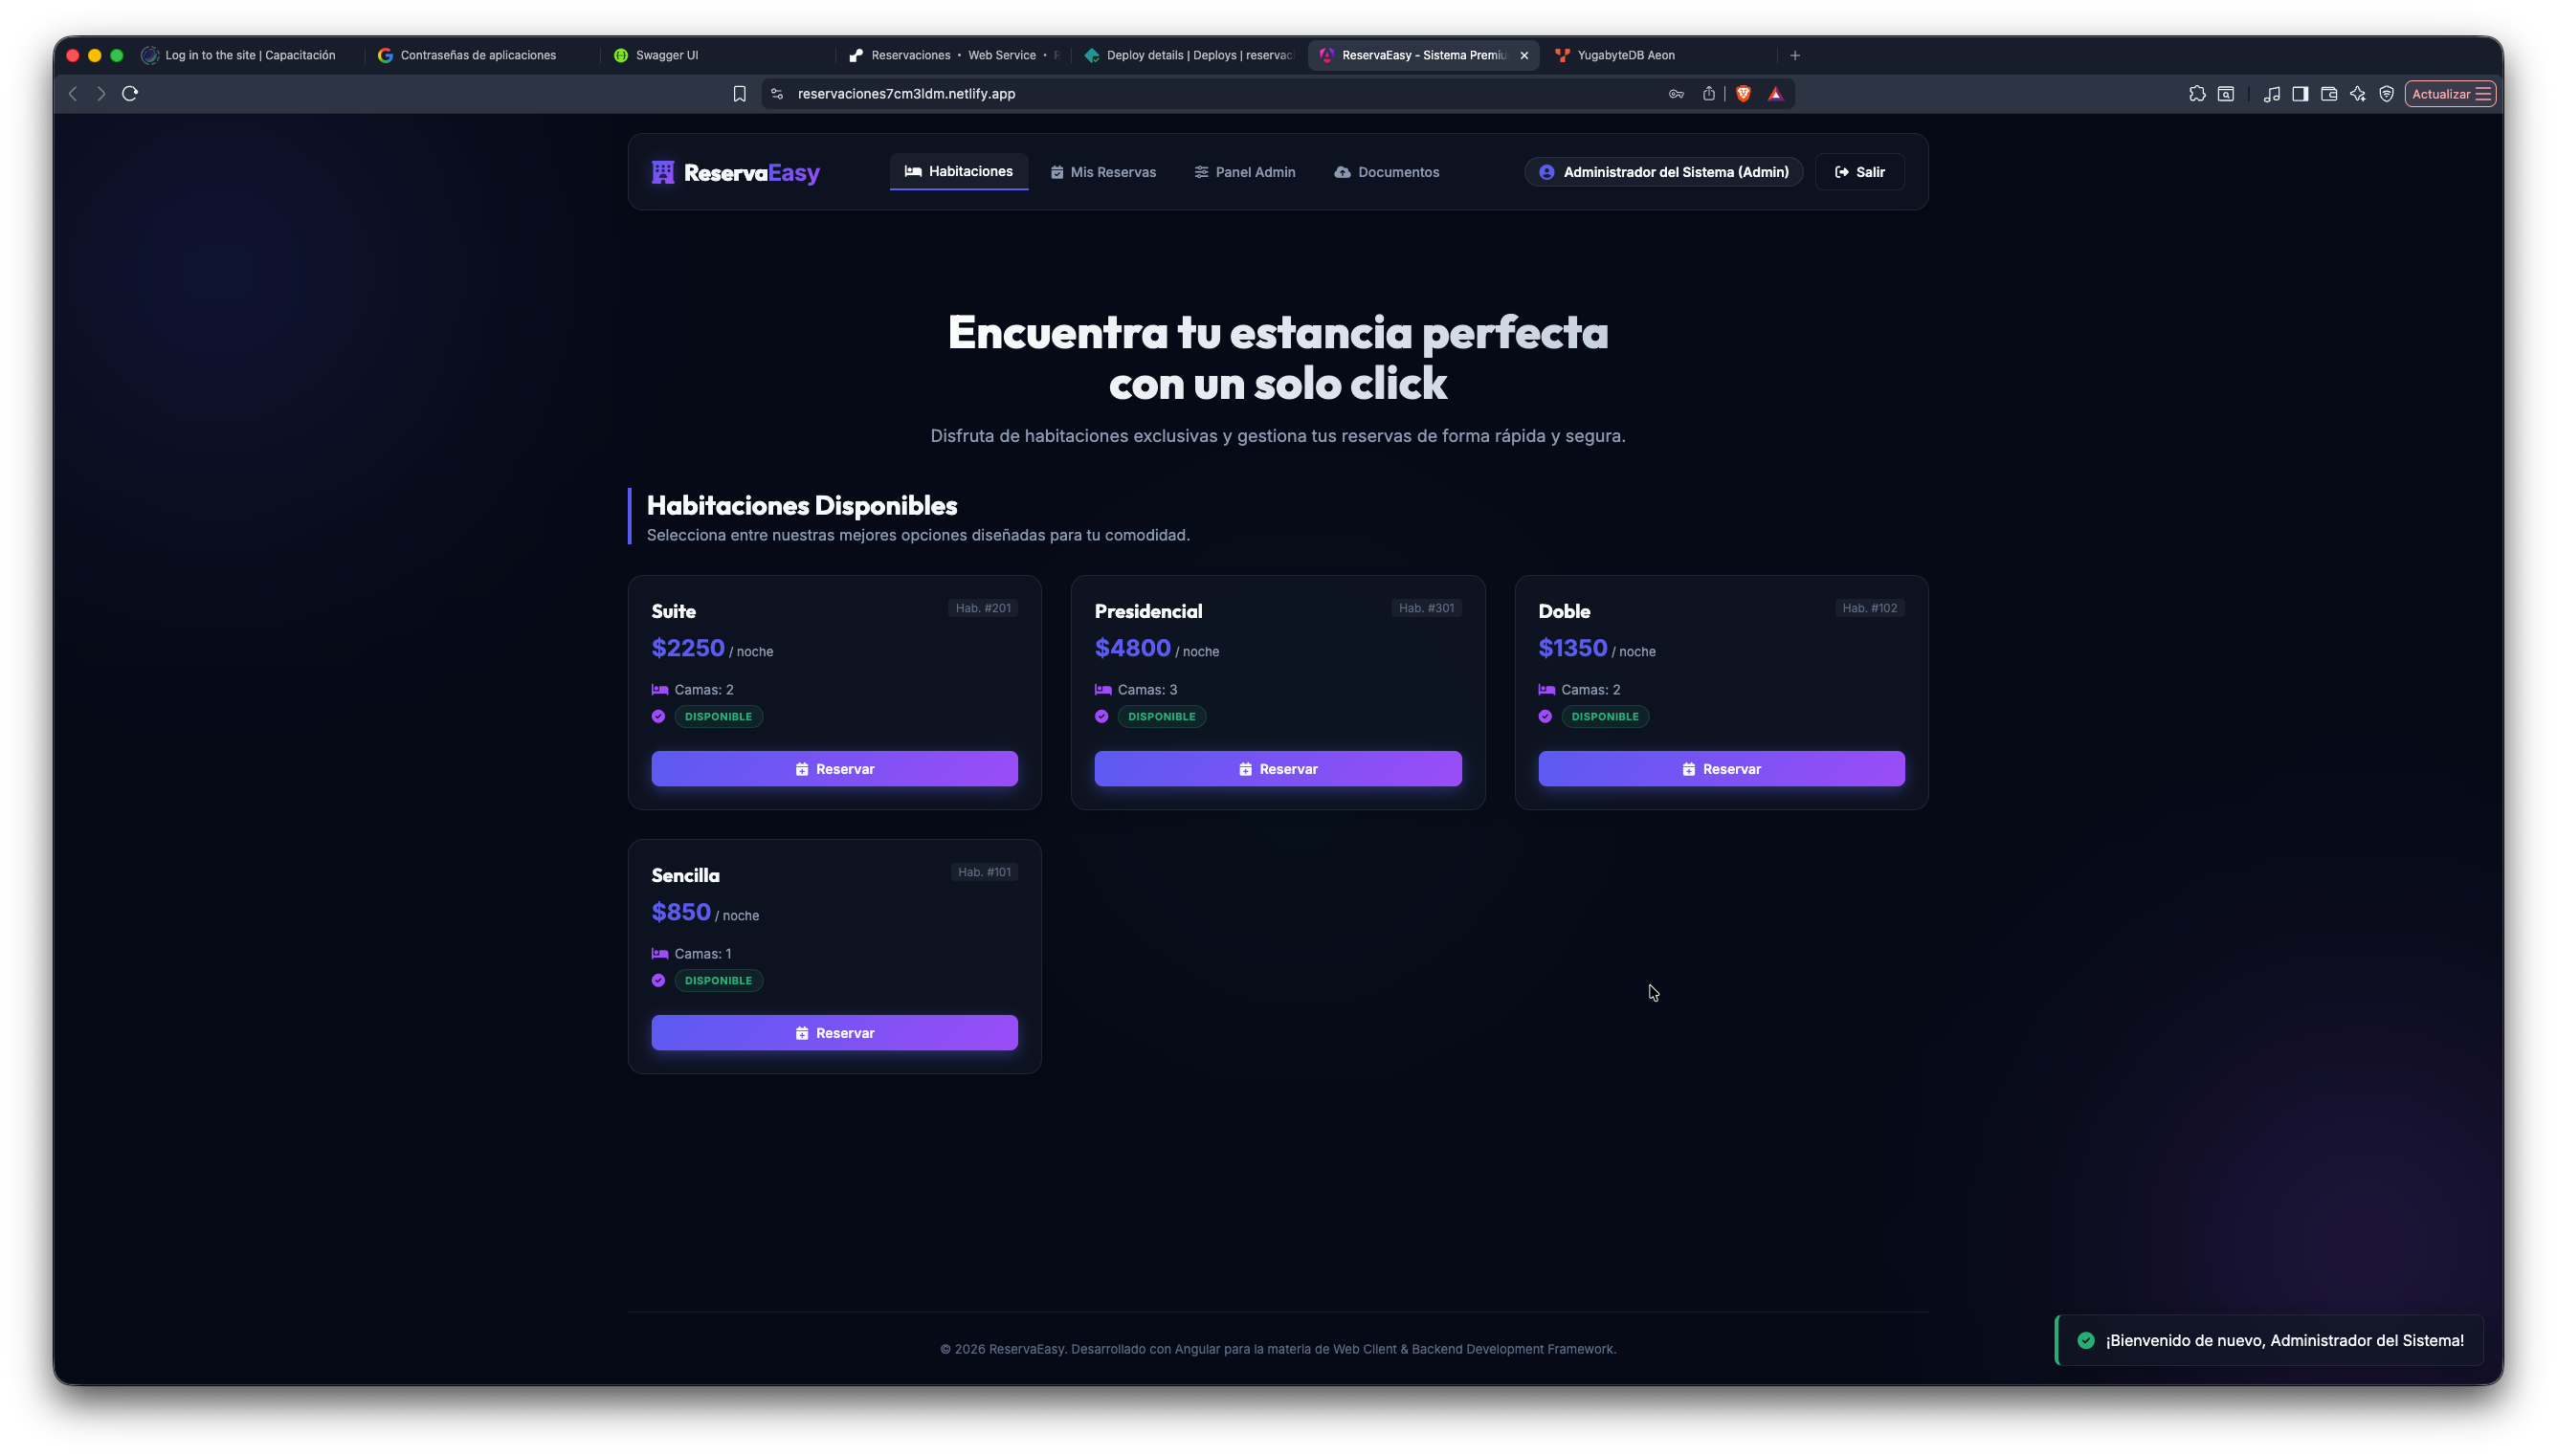
\includegraphics[width=0.75\linewidth]{frontend_rooms}
    \caption{Visualización del catálogo de habitaciones disponibles en la interfaz web.}
    \label{fig:frontend_rooms}
\end{figure}

Al registrar una reserva, se ejecuta una petición POST al backend. El sistema verifica la disponibilidad del cuarto en las fechas indicadas, calcula el costo total, guarda el registro en la base de datos y envía automáticamente un correo de confirmación.

\begin{figure}[H]
    \centering
    \includegraphics[width=0.75\linewidth]{frontend_bookings}
    \caption{Listado de reservaciones de un cliente autenticado, permitiendo modificar fechas o cancelar.}
    \label{fig:frontend_bookings}
\end{figure}

Si el usuario inicia sesión con una cuenta que tiene el rol de administrador, la interfaz habilita la pestaña ``Panel Admin'', permitiendo agregar habitaciones y ver las reservas de todos los clientes de la base de datos.

\begin{figure}[H]
    \centering
    \includegraphics[width=0.75\linewidth]{frontend_admin}
    \caption{Panel administrativo exclusivo para usuarios con ROLE\_ADMIN.}
    \label{fig:frontend_admin}
\end{figure}

\pagebreak

% ################################################
\section{\color{colorIPN}{Conclusión}}

La integración de una SPA en HTML/CSS/JS con una API robusta en Spring Boot y Spring Security demuestra la viabilidad de arquitecturas desacopladas modernas. El uso de Spring Security con usuarios y roles persistidos permite aislar la lógica de permisos en el Back End, garantizando que el sistema sea seguro incluso ante posibles intentos de vulneración en las vistas del cliente web.

\begin{table}[htb]
    \centering
    \begin{tabular}{p{5cm}|p{2cm}|p{2cm}}\hline \hline
        Criterio     & Puntos  & Realizado \\ \hline \hline
        Reservaciones (Back End)  &  30\%  & 30\% \\ \hline 
        Integración Front/Back    &  25\%  & 25\% \\ \hline 
        Spring Security           &  25\%  & 25\% \\ \hline 
        Persistencia DB           &  10\%  & 10\% \\ \hline 
        Reporte y Documentación   &  10\%  & 10\% \\ \hline
        Total                     &  100\%  & 100\% \\ \hline \hline
    \end{tabular}
    \caption{Criterios de Evaluación Práctica 3}
    \label{tabla:EvaluacionT3}
\end{table}

\color{colorIPN}{
	\begin{flushright}
		\textit{
			Luis David Martínez Martínez
		}
	\end{flushright} \hfill \break
}

\pagebreak

% ################################################
\section{\color{colorIPN}{Referencias Bibliográficas}}
\color{colorESCOM}{
	\begin{thebibliography}{10}
    \bibitem[Spring Security, 2026]{SpringSecDoc}
    Spring Projects.
    \newblock {\em Spring Security Reference Architecture Guide.}
    \newblock Broadcom. Disponible en:\\ 
    \url{https://docs.spring.io/spring-security/reference/}

    \bibitem[CORS MDN, 2026]{MDNCors}
    MDN Web Docs.
    \newblock {\em Cross-Origin Resource Sharing (CORS).}
    \newblock Mozilla Network. Disponible en:\\ 
    \url{https://developer.mozilla.org/en-US/docs/Web/HTTP/CORS}
\end{thebibliography}
}

\end{document}
